\scanpage{151}\mspage{6}
\unsure{formal|formal} \unsure{group|groups} is concentrated in commutative formal groups, discovered it seems by Dieudonné \dots). The question I would like to raise is the generalization to groups in $(n\text{-cat})$, one expects to find noncommutative chain complexes
\diagram{\begin{tikzcd}[ampersand replacement=\&,column sep=small]
L_n\arrow[r,no head,to path={-- (\tikztotarget) -- ++(0.025,0.055)}] \& L_{n-\unsure{,|1}}\arrow[r,no head,to path={-- (\tikztotarget) -- ++(0.025,0.055)}] \& \ldots\arrow[r,no head,to path={-- (\tikztotarget) -- ++(0.025,0.055)}] \& L_1\arrow[r,no head,to path={-- (\tikztotarget) -- ++(0.025,0.055)}] \& L_0\arrow[r] \& 1
\end{tikzcd}}
with additional structures probably of type $\unsure{\Theta|\theta}$, but which ones? It is understood that the topological meaning of these structures is that they express exactly the ``homotopy types truncated in dimension $\leq n$'' of topological groups. \inserted{\unsure{measuring} the homotopy types \unsure{truncated|truncated|truncated \deleted{cated}} in dimension $\leq n+1$ of connected point\unsure{e|e}d topological spaces \dots)}
% Guide of the preceding interlinear addition: its left end is before As-tu.
\figure{\begin{tikzpicture}[x=1cm,y=1cm]
\draw (0,0) .. controls (-0.08,0.30) and (-0.05,0.48) .. (0.20,0.53) .. controls (0.90,0.64) and (2.90,0.47) .. (3.30,0.60) -- (3.32,0.72);
\node[inner sep=0pt] at (0.27,0.38) {\unsure{.}};
\end{tikzpicture}}
Do you have any \unsure{candidates|candidates} to propose?

\figure{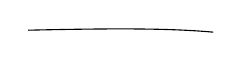
\begin{tikzpicture}\draw (0,0) .. controls (1.1,0.025) and (1.8,0.025) .. (2.35,-0.025);\end{tikzpicture}}

% Guide beneath et d'homologie; the left leg attaches after bidualité.
\figure{\begin{tikzpicture}[x=1cm,y=1cm]
\draw (0,0) -- (0.24,0.64) .. controls (1.20,0.68) and (2.68,0.56) .. (3.45,0.53) -- (3.44,0.65);
\end{tikzpicture}}
\unsure{.} Your reflections on biduality \inserted{and homology}, formal as they may be, are connected with a host of developments, only some of which exist\unsure{,} \unsure{as|as} \unsure{of|of} now, and others would require considerable developments. Here are the reminiscences that your \unsure{naive|naive} questions open up for me:
% archive sheet number: 151
